%%This is a very basic article template.
%%There is just one section and two subsections.
\documentclass[12pt]{article}

\usepackage[margin=0.95in]{geometry}
\usepackage{pdfpages}
\usepackage{indentfirst}
\usepackage{booktabs}
\usepackage{graphicx}
\usepackage{float}
\usepackage{array}
\usepackage{lscape}

%----------------------------------
%------------------------------------------------------
%	TITLE PAGE
%----------------------------------------------------------------------------------------
\newcommand{\tabitem}{~~\llap{\textbullet}~~}

\newcommand*{\titleGP}{\begingroup % Create the command for including the title page in the document
\centering % Center all text
\vspace*{\baselineskip} % White space at the top of the page

\rule{\textwidth}{1.6pt}\vspace*{-\baselineskip}\vspace*{2pt} % Thick horizontal line
\rule{\textwidth}{0.4pt}\\[\baselineskip] % Thin horizontal line

{\LARGE Assignment B2: Behavior Trees\\[0.2\baselineskip]} % Title

\rule{\textwidth}{0.4pt}\vspace*{-\baselineskip}\vspace{3.2pt} % Thin horizontal line
\rule{\textwidth}{1.6pt}\\[\baselineskip]% Thick horizontal line
\vspace{200pt}

\scshape % Small caps
\bf % Tagline(s) or further
% description
{\large Game Documentation\par}
\vspace*{2\baselineskip} % Whitespace between location/year and editors
% description
Intro to Computer Graphics\\
{\itshape Rutgers University}\\[\baselineskip] % Tagline(s) or further 
\vspace*{2\baselineskip} % Whitespace between location/year and editors

Prepared by: \\[\baselineskip]
{\Large Samuel Baysting \\ David Arakelyan \\ Frank Hoffman\par}
 
% Editor list



\vfill % Whitespace between editor names and publisher logo



\endgroup}

%%%%%%%%%%%%%%%%%%%%%%%%%%%%%%%%%%%%%%%%%%%%%%%%%%%%%%%%%%%%%%%%%%%%%
%%%%%%%%%%%%%%%		Begin the Document		%%%%%%%%%%%%%%%%%%%%%%%%%
%%%%%%%%%%%%%%%%%%%%%%%%%%%%%%%%%%%%%%%%%%%%%%%%%%%%%%%%%%%%%%%%%%%%%

\begin{document}
\begin{titlepage}
\pagestyle{empty} % Removes page numbers
\setlength{\parindent}{1cm} % Default is 15pt.

%%%%%%%%%%%%%%%%%%%%%%%%%%%%%%%%%%%%%%%%%%%%%%%%%%%%%%%%%%%%%%%%%%%%%
%%						Title Page
%%%%%%%%%%%%%%%%%%%%%%%%%%%%%%%%%%%%%%%%%%%%%%%%%%%%%%%%%%%%%%%%%%%%%

\titleGP
\end{titlepage}

%%%%%%%%%%%%%%%%%%%%%%%%%%%%%%%%%%%%%%%%%%%%%%%%%%%%%%%%%%%%%%%%%%%%%
%%						Table of Contents
%%%%%%%%%%%%%%%%%%%%%%%%%%%%%%%%%%%%%%%%%%%%%%%%%%%%%%%%%%%%%%%%%%%%%

\newpage
\tableofcontents
\newpage

%%%%%%%%%%%%%%%%%%%%%%%%%%%%%%%%%%%%%%%%%%%%%%%%%%%%%%%%%%%%%%%%%%%%%
%%						Game Details
%%%%%%%%%%%%%%%%%%%%%%%%%%%%%%%%%%%%%%%%%%%%%%%%%%%%%%%%%%%%%%%%%%%%%

\addcontentsline{toc}{section}{Game Details}  
\section*{\center Game Details}
\vspace{10pt}

\subsection*{Movement}

This game uses the mouse to move and interact with the environment via Raycasting. You use LEFT-CLICK (ACTION button) to interact with the other NPCs and the objects in the environment. You use RIGHT-CLICK to move the player around the map.\\ 

\subsection*{Objectives}

Being the police officer in this game, you have three main objectives:

\begin{enumerate}
	\item Rescue the hostages
	\item Kill the criminals
	\item Extinguish the fire
\end{enumerate} 

To do each of these things, you must be close enough to the object/NPC and click the ACTION button. To be able to extinguish the fire, you must first find the fire extinguisher and pick it up. The fire extinguisher spawns in random rooms throughout the house. \\

\newpage

%%%%%%%%%%%%%%%%%%%%%%%%%%%%%%%%%%%%%%%%%%%%%%%%%%%%%%%%%%%%%%%%%%%%%
%%			  Affordance Descriptions
%%%%%%%%%%%%%%%%%%%%%%%%%%%%%%%%%%%%%%%%%%%%%%%%%%%%%%%%%%%%%%%%%%%%%

\addcontentsline{toc}{section}{Affordance Descriptions}  
\section*{\center Affordance Descriptions}
\vspace{10pt}

\subsection*{Cop and Criminal Interaction}

Upon getting close to a criminal and pressing the ACTION button, the cop will perform a motion either pulling out his gun and shooting the criminal or kicking down the criminal. This is random every time. The criminal will then perform a dying motion.\\

\subsection*{Cop and Hostage Interaction}

Upon getting close to a hostage and pressing the ACTION button, the cop will perform a waving-type motion to hurry the hostage out of the room. The hostage will then run out of the room and out of the house. \\

\subsection*{Cop and Outside Person Interaction}

There is a person outside the house that is constantly waving at you. When you approach him and press the ACTION button, the cop will wave at the guy and it will open a dialog that gives you instructions of what to do. The outside guy is randomly performing three different affordances on a loop.\\

\subsection*{Cop and Fire Extinguisher Interaction}

When approaching the fire extinguisher, which spawns randomly in different rooms of the house, and pressing the ACTION button, the cop will bend over and pick up the fire extinguisher. It will then stay in his hand for the rest of the game.\\

\subsection*{Cop and Fire Interaction}

When the cop approaches the fire and presses the ACTION button, if the cop has the fire extinguisher, he will point the extinguisher at the fire and put it out. If he doesn't have the extinguisher, he will do nothing when clicking the fire. You will then have to go and find the extinguisher before putting out the fire.\\
\newpage

%%%%%%%%%%%%%%%%%%%%%%%%%%%%%%%%%%%%%%%%%%%%%%%%%%%%%%%%%%%%%%%%%%%%%
%%			  Affordance Implementations
%%%%%%%%%%%%%%%%%%%%%%%%%%%%%%%%%%%%%%%%%%%%%%%%%%%%%%%%%%%%%%%%%%%%%

\addcontentsline{toc}{section}{Affordance Implementations}  
\section*{\center Affordance Implementations}
\vspace{10pt}

To implement these affordances, we created our own behavior tree for each type of character. Each character behavior file is listed as follows:

\begin{enumerate}
	\item CopBehaviorTree.cs
	\item HostageBehaviorTree.cs
	\item CriminalBehaviorTree.cs
	\item OutsideDudeBehaviorTree.cs
\end{enumerate}

In order to start/stop the animations, we added boolean values to the CharacterMecanim.cs to control who to interact with, what to do while interacting and, most importantly, when to interact. \\

\newpage

%%%%%%%%%%%%%%%%%%%%%%%%%%%%%%%%%%%%%%%%%%%%%%%%%%%%%%%%%%%%%%%%%%%%%
%%			  Custom Animations
%%%%%%%%%%%%%%%%%%%%%%%%%%%%%%%%%%%%%%%%%%%%%%%%%%%%%%%%%%%%%%%%%%%%%

\addcontentsline{toc}{section}{Custom Animations}  
\section*{\center Custom Animations}
\vspace{10pt}

We implemented three custom affordances that weren't in the KADAPT library:

\begin{enumerate}
	\item Pointing extinguisher at the fire
	\item Pulling the gun out
	\item Picking up the object with the left hand
\end{enumerate}

These can be found in the blog and within our implementation of our game.\\

\newpage

%%%%%%%%%%%%%%%%%%%%%%%%%%%%%%%%%%%%%%%%%%%%%%%%%%%%%%%%%%%%%%%%%%%%%
%%			  Behavior Tree Structure
%%%%%%%%%%%%%%%%%%%%%%%%%%%%%%%%%%%%%%%%%%%%%%%%%%%%%%%%%%%%%%%%%%%%%

\addcontentsline{toc}{section}{Behavior Tree Structure}  
\section*{\center Behavior Tree Structure}
\vspace{10pt}

The behavior tree structure for the cop can be found on the illustration in the next page. It includes some essence of randomness, as the project calls for. \\

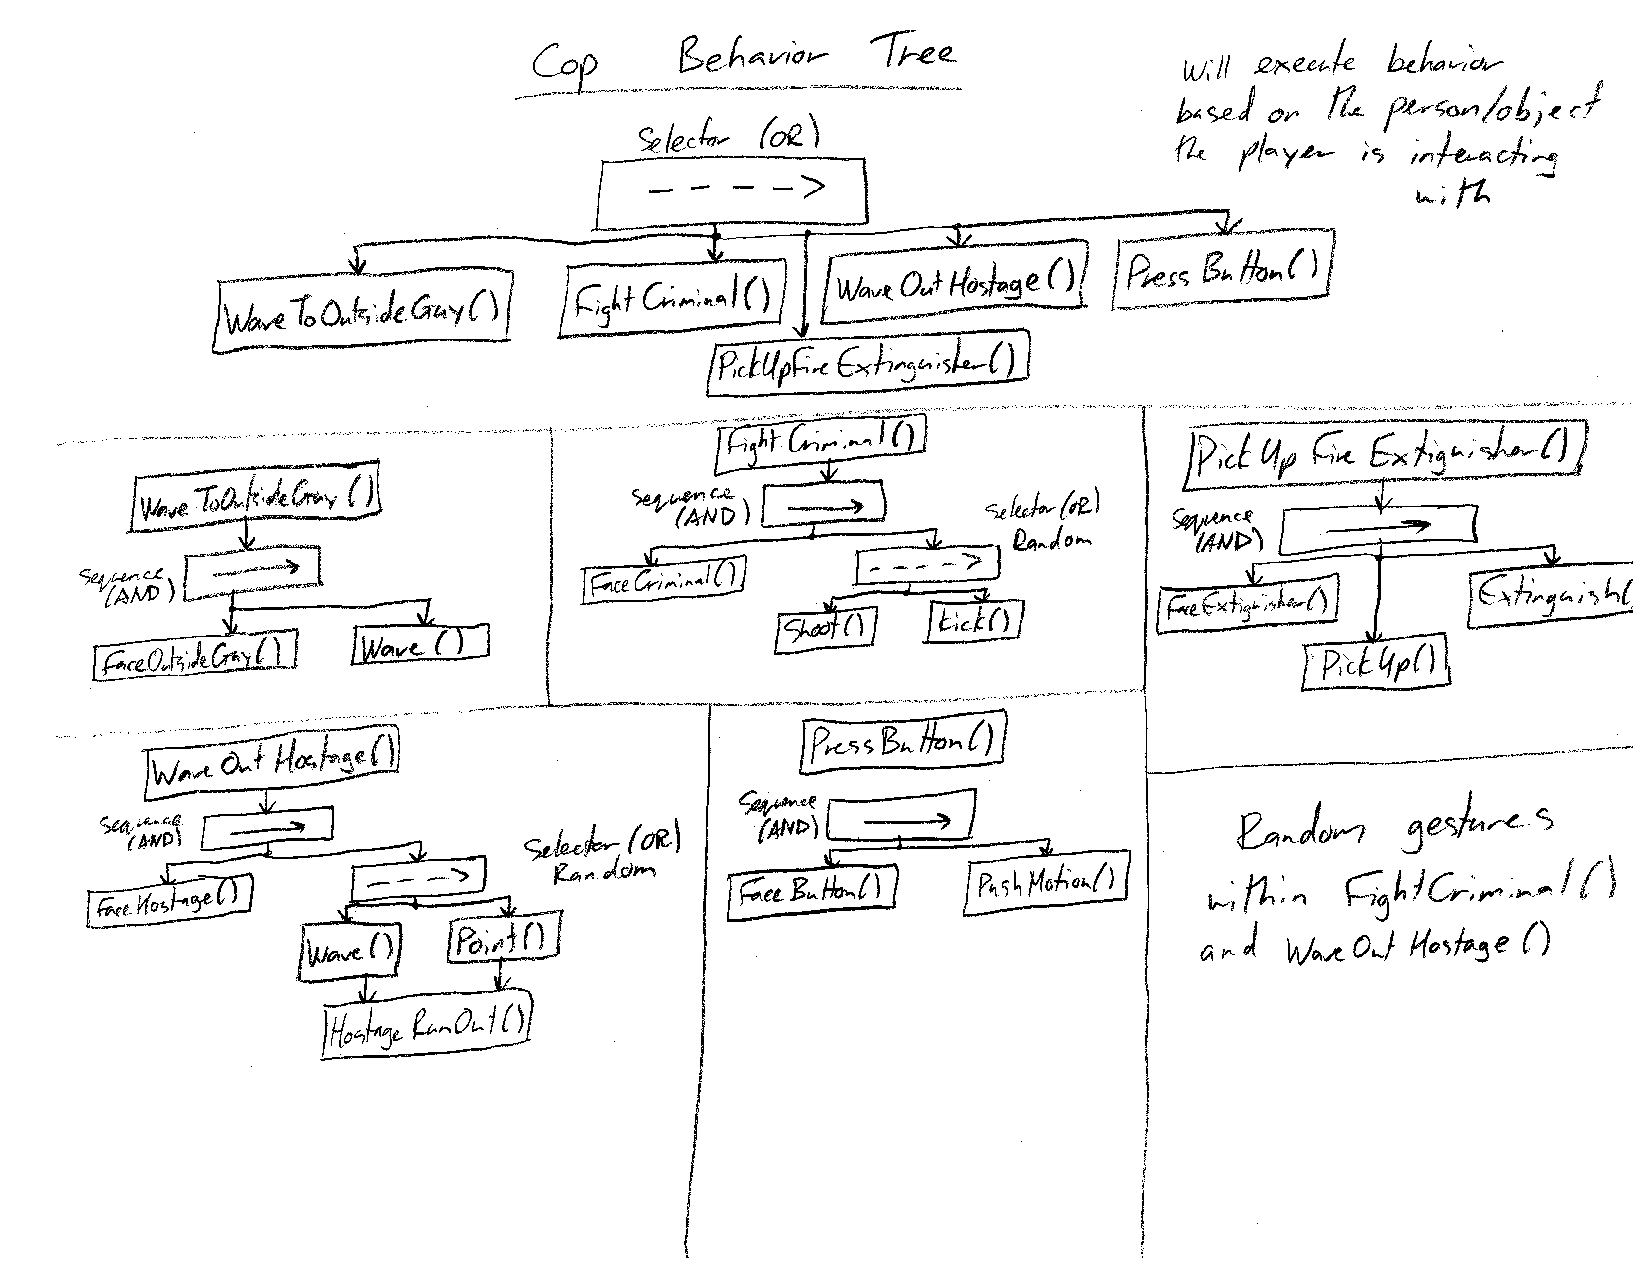
\includepdf{Behavior-Tree-Drawing.pdf}

\newpage

%%%%%%%%%%%%%%%%%%%%%%%%%%%%%%%%%%%%%%%%%%%%%%%%%%%%%%%%%%%%%%%%%%%%%
%%			  Bugs and Relevant Information
%%%%%%%%%%%%%%%%%%%%%%%%%%%%%%%%%%%%%%%%%%%%%%%%%%%%%%%%%%%%%%%%%%%%%

\addcontentsline{toc}{section}{Bugs and Relevant Information}  
\section*{\center Bugs and Relevant Information}
\vspace{10pt}

Our main issue was synchronization of animations. Our animations between characters and objects sometimes have massive delays for an unknown reason. It's probably to do with our implementation of the behaviors and how we activate them. It would be nice to have documentation on KADAPT, because there was none anywhere, making this project extremely difficult.\\


\end{document}